\subsection{LLM-based approach: \qquote{What if an LLM reads the news?}}

One may wonder whether empowering an LLM to parse news articles according to a predefined schema that guides it in ellucidating news-implied firm-specific shocks can deliver better insights on how markets react to new information. In this section we will briefly introduce what Large Language Models are, how they have evolved and then, we will dive into how we can guide them to produce an economically structured analysis of business news. 

%%%%%%%%%%%%%%%%%%%%%%%%%%%%%%%%%%%%%%%%%%%%%%%%%%%%%
%%%%%%%%%%%%%%%%%%%%%%%%%%%%%%%%%%%%%%%%%%%%%%%%%%%%%
\subsubsection{Large Language Models}

In natural language processing (NLP), Large Language Models (LLMs) are designed to \qquote{understand} and generate human-like text. These models utilize the transformer architecture, which excels in modeling complex language tasks by capturing long-range dependencies and contextual relationships.

\mx 
At the heart of LLMs lies the concept of tokens, which serve as the elemental units of text. Tokens can be individual words, subword units, or characters. Let $x_{1:n}:=\3{x_1, x_2, \ldots, x_n}$ represent a sequence of tokens. The goal of an LLM is to estimate the probability distribution of the next token $x_{n+1}$ conditioned on the previous tokens $x_{1:n}$
$$
\P\2{x_{n+1} \mid \3{x_1, x_2, \ldots, x_n}}
.
$$

%\mx 
An LLM is a neural network architecture designed to learn and approximate this conditional probability distribution over sequences of tokens with a large number of parameters $\Theta$. Namely, we can formulate an LLM as a parameterized function $f_{\Theta}$ that maps a sequence of tokens $\3{x_1, x_2, \ldots, x_n}$ to a probability distribution over the vocabulary, where the parameters $\Theta$ are learned from a large corpus of text training data.
$$
f_{\Theta}:\3{x_1, x_2, \ldots, x_n} \rightarrow 
\P\2{x_{n+1} \mid \3{x_1, x_2, \ldots, x_n} ; \Theta}
$$

%\mx 
Interacting with an LLM involves specifying a prefix sequence $x_{1:n}$, termed the \qquote{prompt}, and sampling the subsequent tokens $x_{n+1:z}$, known as the \qquote{completion}. This process enables users to guide and control the generation of text according to desired contexts and constraints.
$$
\ub{\3{x_1,\ldots,x_n}}{\t{prompt}} \longrightarrow \ub{\3{x_{n+1},\ldots,x_z}}{\t{completion}}
$$


\subsubsection{Evolution of LLMs}
The transformer architecture, introduced in the seminal work ``\textit{Attention Is All You Need}'' 
(\cite{vaswani2017attention} Vaswani et al., 2017), 
revolutionized LLM development due to its superior handling of long-range dependencies and efficient parallelization of computations.  Subsequent advancements include the encoder-only \texttt{BERT} model 
(\cite{devlin2018bert} Devlin et al., 2018), 
showcasing the power of pre-training on large datasets for fine-tuning on specific tasks. 

\mx 
Conversely, OpenAI's \texttt{GPT} series 
(\cite{radford2018improving} Radford et al., 2018) 
demonstrated the potential of decoder-only models for generative tasks. In particular, the release of \texttt{GPT-3} marked a significant leap in LLM capabilities with its 175 billion parameters and remarkable few-shot learning abilities. This model highlighted the importance of prompt engineering, where carefully crafted prompts can guide model outputs without extensive fine-tuning.  

\mx 
The trend towards open-source models like \texttt{BLOOM} 
(\cite{le2023bloom} Le Scao et al., 2023), \texttt{Mixtral} and Meta's \texttt{Llama} series 
(\citep{touvron2023llama} Touvron et al., 2023)
emphasizes accessibility and transparency in LLM development.  The latest models, including OpenAI's  \texttt{GPT-4o} and \texttt{GPT-o1}, Google's \texttt{Gemini} and \texttt{Mixtral} and \texttt{Gemma}, Anthropic's \texttt{Claude 3.5 Sonnet}, and Meta's \texttt{Llama-3} series
% \texttt{Llama-3}, \texttt{Llama-3.1} and  \texttt{Llama-3.2} 
continue to push boundaries with improved accuracy, multimodal capabilities, and larger context windows.

\subsubsection{Function Calling with Llama-3}

In our endeavor we will employ \texttt{Llama-3}, developed by Meta AI and released on April 18, 2024 %
%
\footnote{
\href{https://ai.meta.com/blog/meta-llama-3/}
{\qquote{Introducing Meta Llama 3: The most capable openly available LLM to date}
[April 18, 2024]}
}
%
. This model has been pre-trained on approximately 15 trillion tokens of text gathered from ``publicly available sources'' and it comes in two sizes: 8 billion and 70 billion parameters. In this application, we will employ the 70B version, which we will access through an API via \texttt{GroqCloud}.

\mx 
Moreover, we will employ a \textit{function calling} approach to streamline the process of interacting with the LLM. This implies prespecifying a set of functions to the LLM that will then be passed through our dataset of news articles to obtain a structured output in \texttt{JSON} format. The formal procedure is thoroughly described in Appendix \cref{alg:function_calling}

\mx 
Each article $i\in\D$ implies a conversation with the LLM. The structure of the conversation implies defining first a ``system message'', which provides a general context and purpose to the model. In our case:

\begin{quote}
\textit{$-$ You are a function calling LLM that analyses business news in Spanish.  \\
$-$ For every article, you must identify the firms directly affected by the news. Do not include every firm mentioned in the article, only include those that are directly affected by the shocks narrated therein. 
\\
$-$ The identified firms must be Spanish and should be publicly listed in the Spanish exchange (their ticker is of the form `TICKER.MC'). Do not include non-Spanish foreign firms. Do not include Spanish firms that are not publicly traded. \\
$-$ For each identified firm, classify the shocks that affect them (type, magnitude, category). The type of shock can be `demand', `supply', `financial', `policy', or `technology'. The magnitude can be `minor' or `major'. The direction can be `positive' or `negative'. \\
$-$ If a firm is affected neutrally by the news article, don't include it in the analysis.
}
\end{quote}

Then, a news article is fed to the LLM. For illustration purposes, we will work with Example \ref{news:article-cellnex-telefonica}:

%%%%%%%%%%%%%%% ENGLISH VERSION %%%%%%%%%%%%%%%%%%%
\begin{news}
[An article about Cellnex and Telef�nica (translated into English)]
[news:article-cellnex-telefonica]
{Cellnex will face more competition in Europe}
Telef�nica's (TEF.MC) subsidiary, Telxius Telecom, has agreed to sell its telecommunications tower division in Europe and Latin America to American Tower (AMT), which will expand the latter's presence in Europe and increase competition for the Spanish wireless telecommunications group Cellnex Telecom (CLNX.MC), according to Equita Sim. The transaction "represents the entry of a new independent tower operator into the Spanish market and potentially more competition for future growth in the European market as well," says the brokerage firm.		
\end{news}

Next, we define an umbrella function \qquote{firms}, which asks the LLM to identify the set $\F^i_{LLM}$ for each $i\in\D$. Then, for each $j\in\F_{LLM}^i$ we ask the LLM to categorize the type, expected magnitude, and expected direction that the shock described in the article implies in that particular firm $j$.
%----------------------------------------------------
\inserthere{tab:function_calling_structure}

\begin{table}[H]
\centering
\begin{threeparttable}
\caption{Function calling schema}
%{\footnotesize
%\renewcommand{\arraystretch}{1}
\begin{tabular}{lL{4.1cm}L{6.8cm}L{5cm}}
%%%%%%%%%%%%%%%%%%%%%%%%%%%%%%%%%%%%%%%%%%%%%%%%%%%%%
%%%%%%%%%%%%%%%%%%%%%%%%%%%%%%%%%%%%%%%%%%%%%%%%%%%%%
\hline \Xhline{2\arrayrulewidth}
%\rowcolor{gray!10}
\multicolumn{2}{l}{\textbf{Function}} & \textbf{Prompt} & \textbf{Options} \tabularnewline
\hline \Xhline{2\arrayrulewidth} 
\multicolumn{2}{l}{1. \texttt{firms}} & \qquote{List all the firms affected by the events narrated in the article} & \texttt{array} \tabularnewline
\hline
 & 1.1. \texttt{firm} & \qquote{Iterate over each \textnormal{\texttt{firm}} in \textnormal{\texttt{firms}}} & \texttt{string}
 \tabularnewline
\cline{2-4} \cline{3-4} \cline{4-4} 
 & 1.2. \texttt{ticker} & \qquote{State the stock market ticker of \textnormal{\texttt{firm}} } & \texttt{string}
 \tabularnewline
\cline{2-4} \cline{3-4} \cline{4-4} 
 & 1.3. \texttt{shock\_type} & \qquote{What type of shock does this article imply on \textnormal{\texttt{firm}} ?} & \{demand, supply, financial, \newline technology, policy\}\tabularnewline
\cline{2-4} \cline{3-4} \cline{4-4} 
 & 1.4. \texttt{shock\_magnitude} & \qquote{How much impact is this shock expected to have on \textnormal{\texttt{firm}}?} & \{minor, major\}\tabularnewline
\cline{2-4} \cline{3-4} \cline{4-4} 
 & 1.5. \texttt{shock\_direction} & \qquote{In what direction is this shock expected to impact \textnormal{\texttt{firm}}?} & \{positive, negative\}\tabularnewline 
%\cline{2-4} \cline{3-4} \cline{4-4} 
\hline \Xhline{2\arrayrulewidth}
\end{tabular}
%}
%\begin{tablenotes}
%\footnotesize
%\mx
%\item \textit{Note: 
%For clarity of exposition, the actual prompts passed to LlaMA are avoided here but can be found in the code. 
%The ``Options'' column imposes the asnwer format that the LLM must follow. For example, in \texttt{firms}, the option \texttt{array} indicates that the answer must be an enumeration of firms, while the option \texttt{string} in the subfunctions \texttt{firm} and \texttt{ticker} indicates that the answer must be a single name. Finally, the \texttt{shock\_} subfunctions ask the LLM to choose from a predefined set of options.
%}
%\end{tablenotes}
\label{tab:function_calling_structure}
\end{threeparttable}
\mx 
\subcaption*{\textit{
This table outlines the structure of the function calling schema we designed to guide the LLM through the analysis of news-implied firm-specific economic shocks. The \qquote{Function} column specifices the name of the tool passed to the LLM. We can understand the umbrella function \texttt{firms} as running a loop over each of its arguments, with the indented subfunctions being referred to the specific argument passed to them. The \qquote{Prompt} column provides an example of the simplified instructions given to the LLM (the actual prompts are longer as the LLM needs clear and detailed instructions, with useful examples for context).  Finally, the ``Options'' column imposes the answer format that the LLM must follow. For example, in \texttt{firms}, the ``\texttt{array}'' option indicates that the answer must be an enumeration of firms, while the  ``\texttt{string}'' option in the subfunctions \texttt{firm} and \texttt{ticker} indicates that the answer must be a single string. Finally, the \texttt{shock\_} subfunctions ask the LLM to choose from a predefined set of possible responses.
}}
\end{table}



%%%%%%%%%%%%%%%%%%%%%%%%%%%%%%%%%%%%%%%%%%%%%%%%%%%%%
%%%%%%%%%%%%%%%%%%%%%%%%%%%%%%%%%%%%%%%%%%%%%%%%%%%%%

%\begin{table}[H]
%\centering
%\begin{threeparttable}
%\caption{Function calling schema}
%{\small
%\begin{tabular}{l||L{4.1cm}|L{6.8cm}|L{5cm}|}
%%%%%%%%%%%%%%%%%%%%%%%%%%%%%%%%%%%%%%%%%%%%%%%%%%%%%%
%%%%%%%%%%%%%%%%%%%%%%%%%%%%%%%%%%%%%%%%%%%%%%%%%%%%%%
%\hline 
%\multicolumn{2}{|l|}{Function} & Description & Options \tabularnewline
%\hline 
%\hline 
%%\multicolumn{2}{|l|}{1. \texttt{publication\_time}} & Date and time of publication & ``''\tabularnewline
%%\hline 
%%\multicolumn{2}{|l|}{2. \texttt{scope}} & Scope or focus of the news article's impact. & \{Firm, Industry, Economy\}\tabularnewline
%%\hline 
%%\multicolumn{2}{|l|}{3. \texttt{news\_category}} & Type of information provided in the article & \{New, Historical, \newline Analysis/Comments\}\tabularnewline
%%\hline 
%\multicolumn{2}{|l|}{1. \texttt{firms}} & List all the firms affected by the events narrated in the article & \texttt{array} \tabularnewline
%\hline
% & 1.1. \texttt{firm} & Iterate over each firm in \texttt{firms} & \texttt{string}
% \tabularnewline
%\cline{2-4} \cline{3-4} \cline{4-4} 
% & 1.2. \texttt{ticker} & State the stock market ticker of this firm & \texttt{string}
% \tabularnewline
%\cline{2-4} \cline{3-4} \cline{4-4} 
% & 1.3. \texttt{shock\_type} & What type of shock does the article imply on this firm? & \{demand, supply, financial, \newline technology, policy\}\tabularnewline
%\cline{2-4} \cline{3-4} \cline{4-4} 
%% & 4.4. \texttt{shock\_duration} & Expected duration of the shock on this firm & \{Short term, Mid term, Long term\}\tabularnewline
%\cline{2-4} \cline{3-4} \cline{4-4} 
% & 4.5. \texttt{shock\_magnitude} & How much imapct is the shock expected to have on this firm? & \{minor, major\}\tabularnewline
%\cline{2-4} \cline{3-4} \cline{4-4} 
% & 4.6. \texttt{shock\_direction} & In what direction is the shock expected to impact this firm? & \{positive, negative\}\tabularnewline 
%\cline{2-4} \cline{3-4} \cline{4-4} 
%% & 4.6. \texttt{trading\_signal} & Trading decision on this firm's stock & \{Long, Not trade, Short\}\tabularnewline
%%\cline{2-4} \cline{3-4} \cline{4-4} 
%% & 4.7. \texttt{market\_timing} & Time of incorporation of the shock on this firm's stock price (\textit{today=publication date}). & \{Before last week, Last week, \newline Yesterday, Today, Tomorrow, \newline Next week, After next week\}\tabularnewline
%%\cline{2-4} \cline{3-4} \cline{4-4} 
%%%%%%%%%%%%%%%%%%%%%%%%%%%%%%%%%%%%%%%%%%%%%%%%%%%%%%
%%%%%%%%%%%%%%%%%%%%%%%%%%%%%%%%%%%%%%%%%%%%%%%%%%%%%%
%\end{tabular}
%}
%\begin{tablenotes}
%\footnotesize
%\mx
%%\item \textit{Note}: A justification of the category choice is asked for all the parameters with an asterisk . 
%\item \textit{Note: For clarity of exposition, the actual prompts passed to Llama are avoided here but can be found in the Appendix. The ``Options'' column imposes the asnwer format that the LLM must follow. For example, in \texttt{firms}, the option \texttt{array} indicates that the answer must be an enumeration of firms}, while the option \texttt{string} in the subfunctions \texttt{firm} and \texttt{ticker} indicates that the answer must be a single name. Finally, the shock subfunctions ask the LLM to choose an option from a predefined set of options.
%\end{tablenotes}
%\end{threeparttable}
%\end{table}
%----------------------------------------------------

The function calling schema is outlined in \cref{tab:function_calling_structure}. First, we need to prompt the LLM, and then we need to specify the desired format of its response. The ``Options'' column imposes the answer format that the LLM must follow. For example, in \texttt{firms}, the ``\texttt{array}'' option indicates that the answer must be an enumeration of firms, while the  ``\texttt{string}'' option in the subfunctions \texttt{firm} and \texttt{ticker} indicates that the answer must be a single name. Finally, the \texttt{shock\_} subfunctions ask the LLM to choose from a predefined set of possible responses.

\mx 
Note that the firms identified by the LLM are used to validate the firms identified by the pattern recognition algorithm (those extracted with \texttt{regex} by exploiting the pattern \texttt{<WORD>.MC}). As mentioned earlier, given the high quality of the filtered dataset (the ticker of the firms that are actively involved in the article are explicitly stated), they are almost identical. Hence, we indistinctively use $\F_i$ to simplify notation.

\mx 
The LLM provides two outputs: structured data (\qquote{Structured Output}) and a explanatory text describing its reasoning (\qquote{Unstructured Ouptut}). The explanations help us verify if the model correctly understands how to use the function-calling schema and follow system instructions. 
To assess the LLM's understanding, we review a random sample of these explanations and look for patterns of misinterpretation, confusion, or hallucination. If we identify such issues, we refine the system prompts and function descriptions to provide clearer guidance. This iterative prompt refinement continues until the LLM reliably generates correct outputs across multiple test scenarios. 

\begin{quote}

\textbf{1) Structured Output: } 

\vspace{0.2cm}
{\centering
	\begin{tabular}{ccccc}
		\hline \Xhline{2\arrayrulewidth}
		\texttt{firm} & \texttt{ticker} & \texttt{shock\_type} & \texttt{shock\_magnitude} & \texttt{shock\_direction}
		\\ \hline \Xhline{2\arrayrulewidth} 
		Cellnex Telecom & CLNX.MC & supply & minor & negative
		\\ 
		Telef�nica & TEF.MC & financial & minor & positive
		\\ 
		\hline \Xhline{2\arrayrulewidth}
	\end{tabular}
\par}
\vspace{0.2cm}

\textbf{2) Unstructured Output (justification)}

\textit{The news about American Tower's expansion in Europe may increase competition for Cellnex, which is why it's classified as a negative supply shock. On the other hand, Telef�nica benefits from the sale of its tower division, which is why it's classified as a positive financial shock.}

\end{quote}

This procedure is run iteratively from beginning (defining system prompt) to end (getting the output) for every $i\in\D$.\footnote{
This procedure was run on a MacBook Pro M2 with 16GB RAM, 12-core central processing units (CPU), 19-core graphics processing units (GPU), and 16-core Neural Engine. 
%The first run of the code takes about 18.4 hours; however, successive runs were required afterwards with smaller subsets of failed articles, as the LLM always raises errors for a certain percentage of the articles that are fed to it.
}

%%%%%%%%%%%%%%%%%%%%%%%%%%%%%%%%%%%%%%%%%%%%%%%%%%%%%
%%%%%%%%%%%%%%%%%%%%%%%%%%%%%%%%%%%%%%%%%%%%%%%%%%%%%

\subsubsection{Clustering with the LLM}
Formally, we can define the set $\mathcal B:=\{(i,j)\mid i\in \D ~\wedge~j\in\mathcal F^i \}$ containing all the unique pairs of articles and identified firms. 
The LLM assigns each pair $(i,j)\in \mathcal B$ with a choice from each of the following sets:
$$
\begin{array}{llll}
\t{\qquote{shock type}}
&& \mathcal{S}_T
& := \{\t{demand, supply, financial, technology, policy}\}
\\[0.3em]
\t{\qquote{shock magnitude}}
&& \mathcal{S}_M
& :=\{\t{minor, major}\} 
\\[0.3em]
\t{\qquote{shock direction}}
&& \mathcal{S}_D
& := \{\t{positive, negative}\}
\end{array}
$$
The clustering of news articles follows naturally by taking the Cartesian product of these three sets:
$
\mathcal{G}_{LLM} := \mathcal{S}_T \times \mathcal{S}_M \times \mathcal{S}_D
,
$
and the total number of clusters is now $k_{LLM} =|\mathcal{G}_{LLM}|=20$. 
Consequently, a news article to which the LLM assigns $s_T\in\mathcal{S}_T$, $s_M\in\mathcal{S}_M$, $s_D\in\mathcal{S}_D$ will belong to cluster $(s_T,s_M, s_D)\in \mathcal{G}_{LLM}$. Formally, the set of all possible clusters is defined as: 
$$
\mathcal{G}_{LLM} := \3{(s_T,s_M, s_D) \c  s_T\in\mathcal{S}_T, s_M\in\mathcal{S}_M, s_D\in\mathcal{S}_D}
,
$$
and each cluster can then be mapped to a positive integer as $\mathcal G_{LLM}\to \{k\in \mathbb{N}_0 \mid 0\leq k\leq 19\}$.
A representative sample of 3 articles from each cluster is provided in Appendix \cref{tab:LLM_Articles_3_English}. 

%%%%%%%%%%%%%%%%%%%%%%%%%%%%%%%%%%%%%%%%%%%%%%%%%%%%%
\mx 
In \cref{fig:LLM_cluster_distribution} we plot the distribution of news articles through clusters. As we can see, most articles are assigned to clusters 8, 9, 10, and 11, which are the clusters referred to financial events or shocks. Such clusters are mostly composed of articles about the publication of quarterly and semiannual results. More specifically, cluster 8 (\textit{financial, minor, positive}) concentrates around 1/3 of the sample and is associated to the publication of results that mildly surpass the expectations of investors, hence, making this cluster a good candidate for a long trading signal.

\mx 
On the other hand, other clusters such as 16 (\textit{policy, minor, positive}) and 0 (\textit{demand, minor, positive}) also concentrate a big share of news. Note that no cluster has been assigned to cluster 13 (\textit{technology, minor, negative}).
%
Compared to KMeans clustering with embeddings, the distribution of articles across these refined clusters is now remarkably stable across different data splits. This consistency indicates that clustering based on a thorough analysis of the shocks implied by each article for the affected firms yields a robust, time-invariant categorization. This is an encouraging finding for subsequent research and applications.

%----------------------------------------------------
%----------------------------------------------------
\inserthere{fig:LLM_cluster_distribution}
\begin{figure}[H]
    \centering
    \caption{Distribution of articles through LLM clusters}
    
    % Upper plot
    \begin{subfigure}[b]{\textwidth}
        \caption{All data ($\mathcal D$)}
        \centering
        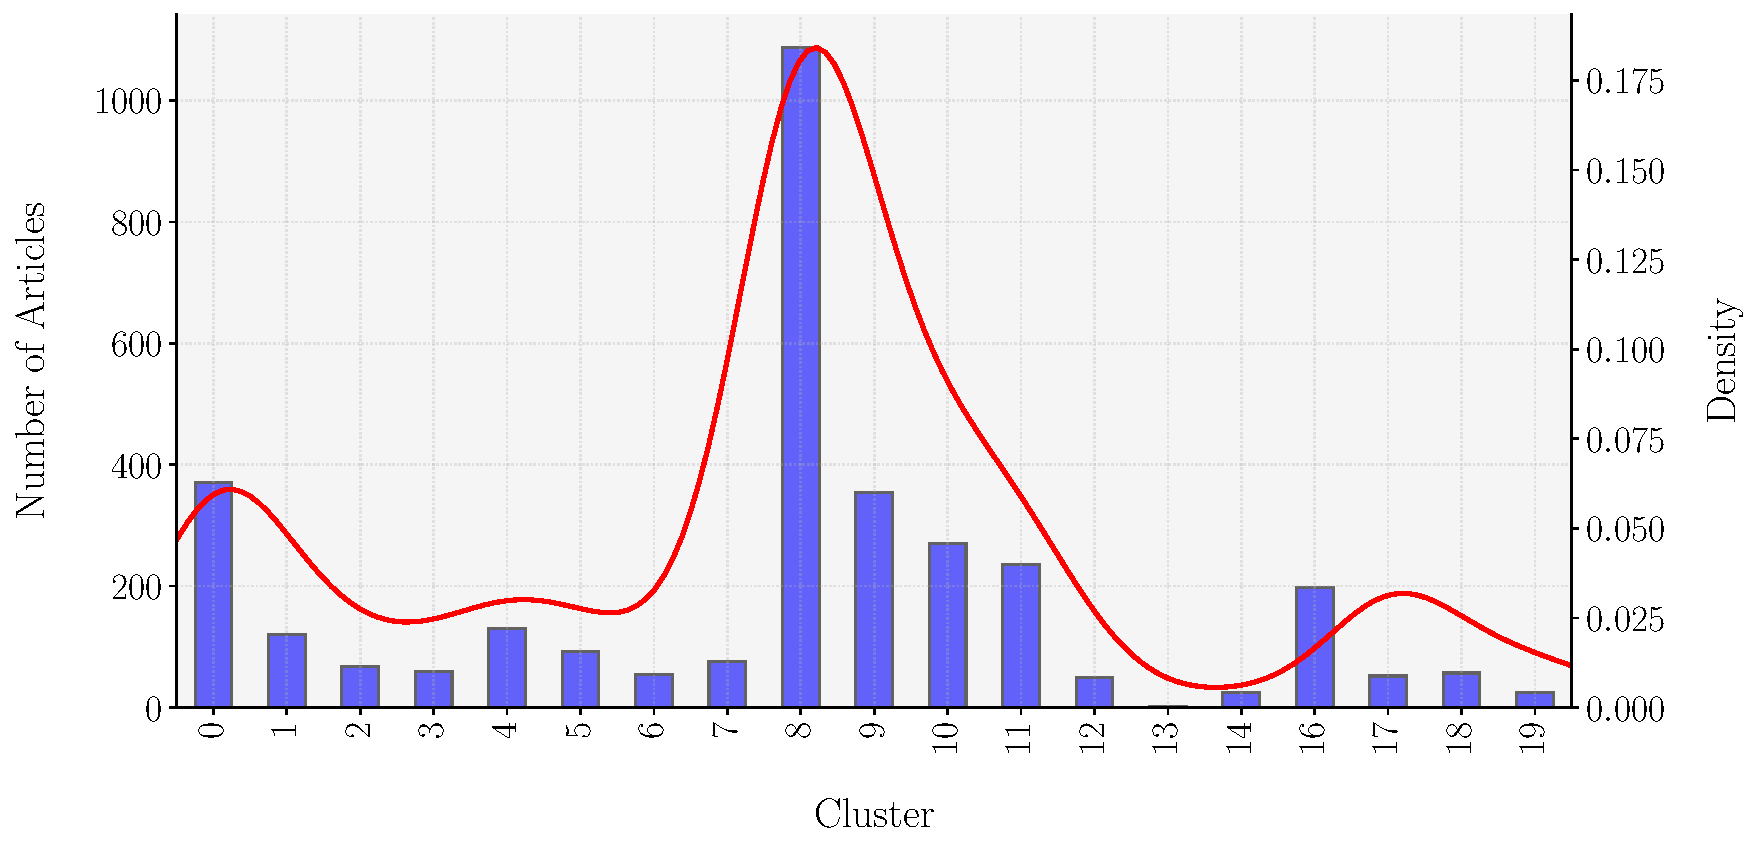
\includegraphics[scale=0.48]{fig_6a_LLAMA_Cluster_Distribution.pdf}
        \label{fig:all_data}
    \end{subfigure}

    % Lower plots
    \begin{subfigure}[b]{0.32\textwidth}
        \caption{Training data ($\D^{tr}$)}
        \centering
        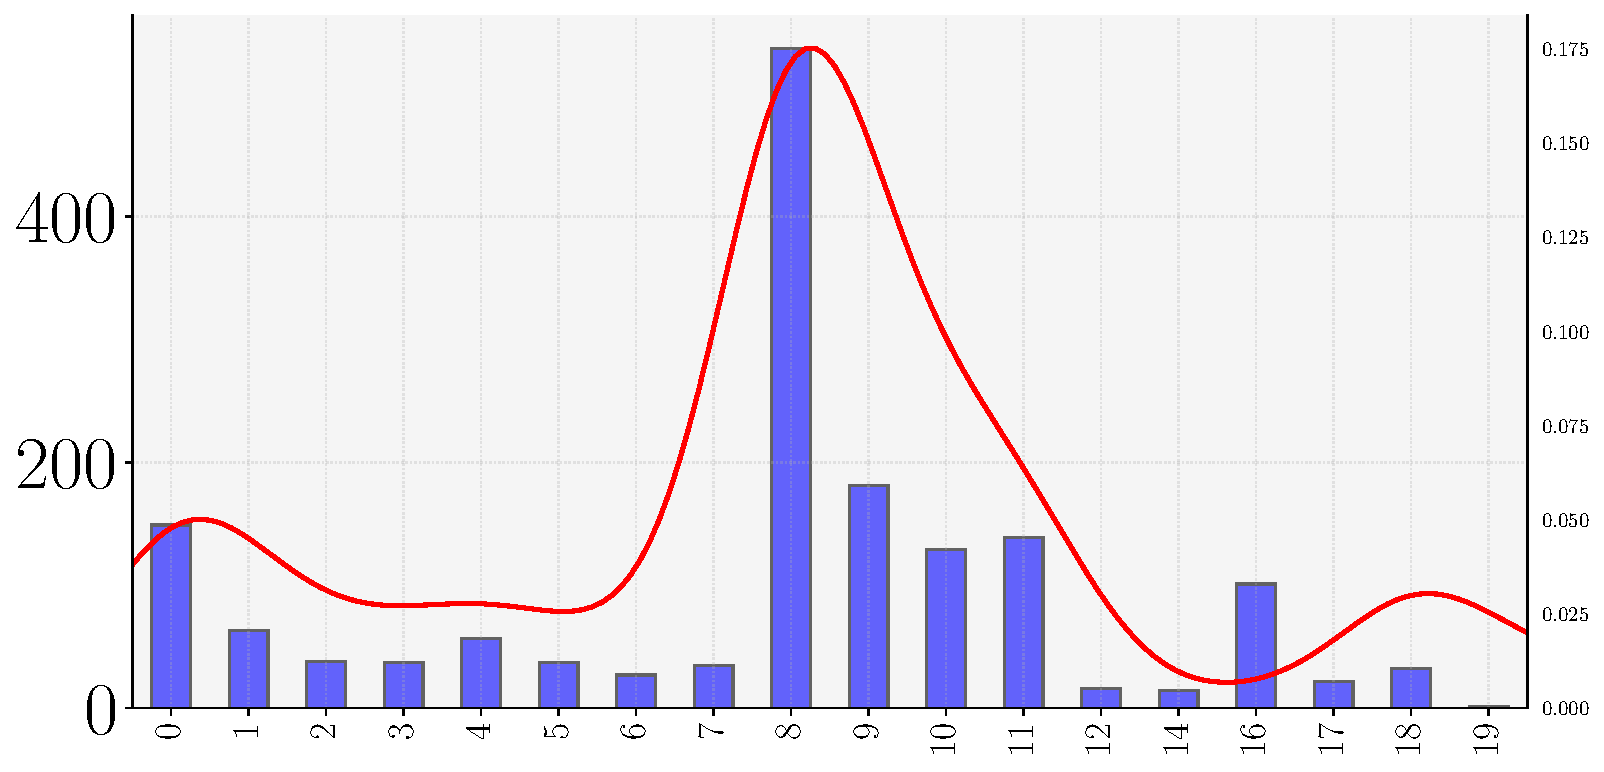
\includegraphics[width=\textwidth]{fig_6b_LLAMA_Cluster_Distribution_Train.pdf}
        \label{fig:train_data}
    \end{subfigure}
    \begin{subfigure}[b]{0.32\textwidth}
        \caption{Validation data ($\D^{val}$)}
        \centering
        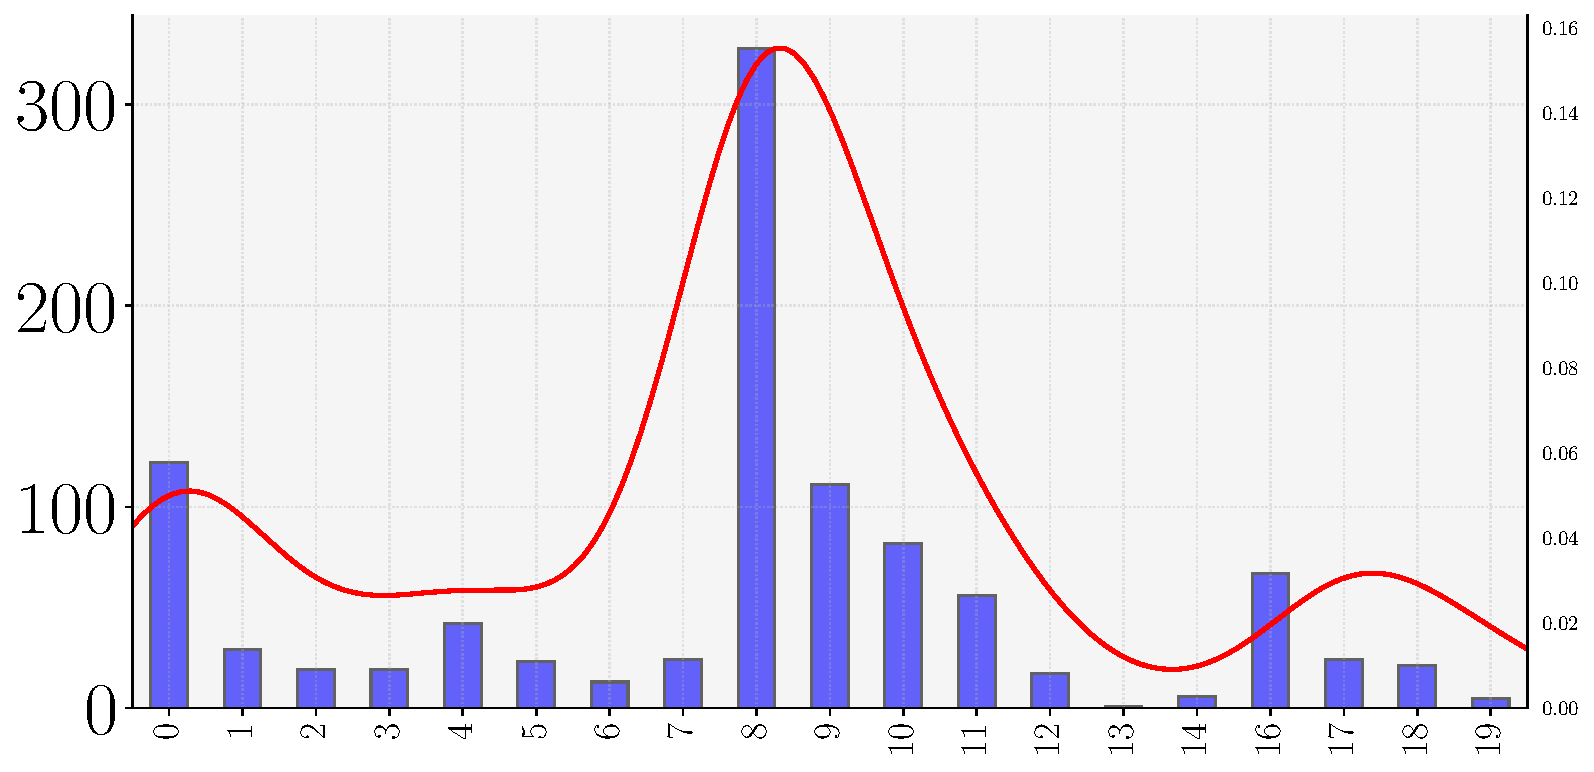
\includegraphics[width=\textwidth]{fig_6c_LLAMA_Cluster_Distribution_Validation.pdf}
        \label{fig:val_data}
    \end{subfigure}
    \begin{subfigure}[b]{0.32\textwidth}
        \caption{Test data ($\D^{test}$)}
        \centering
        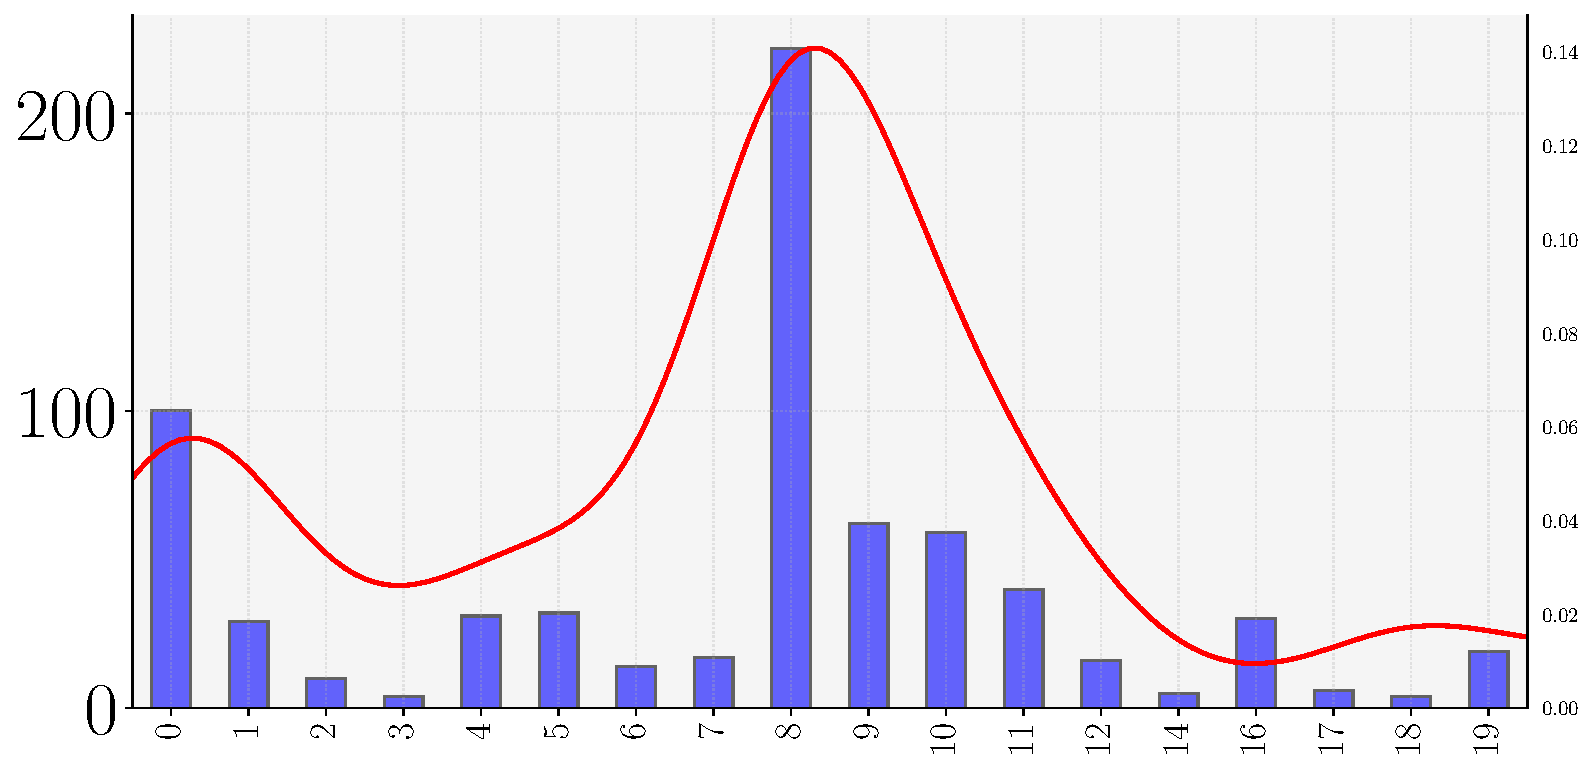
\includegraphics[width=\textwidth]{fig_6d_LLAMA_Cluster_Distribution_Test.pdf}
        \label{fig:test_data}
    \end{subfigure}
    \label{fig:LLM_cluster_distribution}
    \subcaption*{\textit{Note: This figure presents the distribution of news articles across clusters derived using an LLM-based approach. The upper plot shows the distribution for the entire dataset ($\mathcal D$), while the lower plots display the distributions for the training ($\D^{tr}$), validation ($\D^{val}$), and test ($\D^{test}$) datasets. Clusters 8, 9, 10, and 11, which capture financial events or shocks, dominate the distribution, with cluster 8 (\textit{financial, minor, positive}) representing approximately one-third of the dataset. This cluster includes articles related to financial reports with mildly positive outcomes, potentially offering insight for long trading signals. Unlike KMeans clustering with embeddings, this LLM-based clustering shows stable distributions across data splits, highlighting the robustness of this method over time. }}
\end{figure}
%----------------------------------------------------
%----------------------------------------------------

